\begin{activity}\label{A:0.3.3}
    \ba
        \item Based on symmetry alone, is $f(x) = x^2$ an even or an odd function?
        \item Based on symmetry alone, is $g(x) = x^3$ an even or an odd function?
        \item Find $f(-x)$ and $g(-x)$ and make conjectures to complete these sentences:
            \begin{itemize}
                \item If a function $f(x)$ is \underline{even} then $f(-x) =
                    $\underline{\hspace{1in}}.
                \item If a function $f(x)$ is \underline{odd} then $f(-x) =
                    $\underline{\hspace{1in}}.
            \end{itemize}
            Explain why the composition $f(-x)$ is a good test for symmetry of a function.
        \item Classify each of the following functions as even, odd, or neither.
            \[ h(x) = \frac{1}{x}, \quad j(x) = e^x, \quad k(x) = x^2-x^4, \quad n(x) =
            x^3+x^2. \]
        \item Each figure below shows only half of the function.  Draw the left
            half so $f(x)$ is even.  Draw the left half so $g(x)$ is odd. Draw the left
            half so $h(x)$ is neither even nor odd.
            \begin{center}
%                 \begin{tikzpicture}[scale=0.65]
%                     \draw[color=gray] (-3,-3) grid (3,3);
%                     \draw[thick, black, <->] (-3,0) -- (3,0) node[anchor=west]{$x$};
%                     \draw[thick, black, <->] (0,-3) -- (0,3) node[anchor=west]{$x$};
%                     \draw[very thick, blue] (0,0) -- (1,1) -- (2,1) -- (3,-1)
%                     node[anchor=north]{$f(x)$}; 
%                 \end{tikzpicture}
%                 \begin{tikzpicture}[scale=0.65]
%                     \draw[color=gray] (-3,-3) grid (3,3);
%                     \draw[thick, black, <->] (-3,0) -- (3,0) node[anchor=west]{$x$};
%                     \draw[thick, black, <->] (0,-3) -- (0,3) node[anchor=west]{$x$};
%                     \draw[very thick, blue] (0,0) -- (1,1) -- (2,1) -- (3,-1)
%                     node[anchor=north]{$g(x)$}; 
%                 \end{tikzpicture}
%                 \begin{tikzpicture}[scale=0.65]
%                     \draw[color=gray] (-3,-3) grid (3,3);
%                     \draw[thick, black, <->] (-3,0) -- (3,0) node[anchor=west]{$x$};
%                     \draw[thick, black, <->] (0,-3) -- (0,3) node[anchor=west]{$x$};
%                     \draw[very thick, blue] (0,0) -- (1,1) -- (2,1) -- (3,-1)
%                     node[anchor=north]{$h(x)$}; 
%                 \end{tikzpicture}
                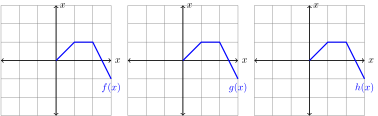
\includegraphics[width=0.9\columnwidth]{figures/0-3-fig4.pdf}
            \end{center}
    \ea
\end{activity}
\begin{smallhint}
   \ba
        \item Draw a plot of the function.  Is there reflective symmetry or rotational
            symmetry?
        \item Draw a plot of the function.  Is there reflective symmetry or rotational
            symmetry?
        \item Put $-x$ into the function and see what results.
        \item Use the test that you devised in part (c)
        \item Think about how to use to the test from part (c) graphically.
   \ea
\end{smallhint}
\begin{bighint}
   \ba
        \item Does the left side line up with the right side of $f(x) = x^2$ when we
            reflect over the $y$ axis or when we rotate about the origin?
        \item Does the left side line up with the right side of $g(x) = x^3$ when we
            reflect over the $y$ axis or when we rotate about the origin?
        \item Notice that $f(-x) = (-x)^2 = x^2$ and $g(-x) = (-x)^3 = -x^3$.
        \item What happens when we evaluate $h(-x)$, $j(-x)$, $k(-x)$, and $n(-x)$?
        \item It may be helpful to fold or rotate your paper.
   \ea
\end{bighint}
\begin{activitySolution}
   \ba
        \item $f(x)=x^2$ is an even function.  If you reflect of the $y$ axis you get a
            perfect match.
        \item $g(x) = x^3$ is an odd fnction.  If you rotate about the origin you get a
            perfect match.
        \item If $f(x)$ is even then $f(-x) = f(x)$.  If $f(x)$ is odd then $f(-x) =
            -f(x)$.
        \item 
            \begin{flalign*}
                h(-x) &= \frac{1}{(-x)} = -\frac{1}{x} = -h(x) \quad \implies \quad
                h(x) \text{ is odd } \\
                j(-x) &= e^{-x} = \frac{1}{e^x} \quad \implies \quad
                j(x) \text{ is neither even nor odd } \\
                k(-x) &= (-x)^2 - (-x)^4 = x^2 - x^4 = k(x) \quad \implies \quad
                k(x) \text{ is even} \\
                n(-x) &= (-x)^3 + (-x)^2 = -x^3 + x^2 \quad \implies \quad
                n(x) \text{ is neither even nor odd }
            \end{flalign*}
        \item See the plot below for the answers to the left and middle plots.  The
            right-hand plot can be anything other than the first two.
            \begin{center}
                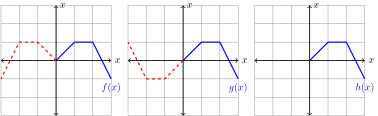
\includegraphics[width=0.9\columnwidth]{figures/0-3-fig4soln.pdf}
            \end{center}
   \ea
\end{activitySolution}

\aftera
